
\chapter*{Introduction\markboth{\bf Introduction}{}}
\label{chap:intro}
\addcontentsline{toc}{chapter}{Introduction}

Deeply virtual Compton scattering on a nucleon is an exclusive process which 
when measured over a broad range of kinematics can be used to extract 
information about the generalized parton distributions (GPDs) of the nucleon.  
The extracted quark and gluon GPDs offer a three dimensional picture of how 
quarks and gluons are distributed in the nucleon. DVCS measurements on the 
proton\cite{Chekanov:2003ya,Camacho:2006qlk} have already begun to provide 
insight into this picture of the nucleon, however, without a free neutron 
target a flavor separation will always require an approximation using a 
deuteron target with some nuclear corrections.  The EMC effect demonstrated 
that medium modifications to the nucleon can be significant for heavy nuclei 
but the degree to which modifications exist in light nuclei is 
unknown.\footnote{Perhaps the earliest known medium modification of the nucleon 
   is the free neutron lifetime compared the significantly longer lifetime when 
bound in a nucleus.} Furthermore, when considering the Fermi motion of a bound 
nucleon in say, deuterium, there exist a probability of finding a nucleon 
moving with large relative momenta which corresponds to a configuration where 
the two nucleons are separated by a small distance.  Although this probability 
is small, hence leading to a small overall contribution to the EMC effect, by 
selecting only these dense configurations through spectator tagging in hard 
processes, sizable modifications of the nucleon can be observed.



This proposal consists of three components: nuclear DVCS, incoherent DVCS, 
unique DVCS breakup reactions. First, a comparison of the DVCS beam spin 
asymmetries on the neutron using deuterium and helium-4 targets representing 
the quasi-free and bound nucleon.

Second we will investigate the incoherent DVCS process on 

The final component of this proposal involves exploring novel DVCS reactions 
where the spectator system 

\begin{figure}
   \centering
   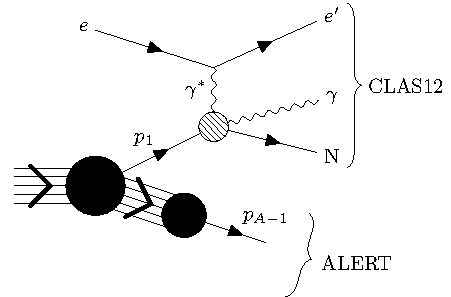
\includegraphics{../tikz/dvcs_feynman/dvcs_feynman-figure0.pdf}
   \caption{\label{fig:taggedDVCS}Tagged DVCS diagram showing the detection of 
   the forward DVCS final state particles in CLAS12 and the detection of the 
recoiling spectator system (A-1) in ALERT.}
\end{figure}


